\documentclass[18pt,xcolor=table]{beamer}

%!TEX root = ./main.tex
\usepackage {bbm}
\usepackage {textpos}
\usepackage {tikz}
\usepackage {graphicx}


\definecolor{blue1}{RGB}{176,196,222 }
\definecolor{blue2}{RGB}{54,100,139}

\definecolor{grey1}{RGB}{139,139,131}
\definecolor{grey2}{RGB}{235,235,235}

\definecolor{black1}{RGB}{50,50,50}

\mode<presentation>
{
  % \usetheme{Pittsburgh}   
  %\usetheme{Boadilla}  
\usetheme{Madrid}  
  \usefonttheme[onlymath]{serif}
  \setbeamertemplate{items}[circle] 
  \setbeamertemplate{sections/subsections in toc}[circle]
  \setbeamercovered{invisible}
  \setbeamertemplate{navigation symbols}{}
% \usecolortheme{seahorse}
%
%  % Color Theme 
  \setbeamercolor{normal text}{bg=white,fg=black1} %All standard text
  \setbeamercolor{structure}{fg=blue2} %% Table of Contents 

  \setbeamercolor*{frametitle}{fg=black1,bg=grey2} % Frame title colors
%  \setbeamerfont{frametitle}{series=\bfseries}
  \setbeamercolor*{framesubtitle}{fg=blue2} % Frame subtitle color

  \setbeamercolor*{palette primary}{use=structure,fg=black1, bg=grey2} %right bottom
  \setbeamercolor*{palette secondary}{use=structure,bg=blue1} %middle bottom
  \setbeamercolor*{palette tertiary}{use=structure,bg=blue2,fg=grey2} %left bottom

  \setbeamercolor*{block body}{fg=black1,bg=blue1!10} % Color of blocks
  \setbeamercolor*{block title}{parent=structure,fg=black1,bg=blue1} % Block Titles
  \setbeamercolor{alerted text}{fg=blue2!85!black,} % Alerted Text (ie. highlight with \alert)
  \setbeamerfont{alerted text}{series=\bfseries}

  % not sure what these do.
  \setbeamercolor{item projected}{use=item,fg=black1,bg=item.fg!35}
  \setbeamercolor*{block title alerted}{parent=alerted text,bg=black1!15}
  \setbeamercolor*{block title example}{parent=example text,bg=black1!15}
  \setbeamerfont{framesubtitle}{size=\small}
}

\makeatletter
\setbeamertemplate{footline}
{
  \leavevmode%
    \hbox{%
      \begin{beamercolorbox}[wd=.333333\paperwidth,ht=2.25ex,dp=1ex,center]{author in head/foot}%
        \usebeamerfont{author in head/foot}\insertshortauthor%~~\beamer@ifempty{\insertshortinstitute}{}{(\insertshortinstitute)}
      \end{beamercolorbox}%
        \begin{beamercolorbox}[wd=.333333\paperwidth,ht=2.25ex,dp=1ex,center]{title in head/foot}%
        \usebeamerfont{title in head/foot}\insertshorttitle
        \end{beamercolorbox}%
        \begin{beamercolorbox}[wd=.333333\paperwidth,ht=2.25ex,dp=1ex,right]{date in head/foot}%
        \usebeamerfont{date in head/foot}\insertshortdate{}\hspace*{2em}
        \insertframenumber{} / \inserttotalframenumber\hspace*{2ex} 
      \end{beamercolorbox}}%
        \vskip0pt%
}
\makeatother

%\usepackage{kerkis}
\usepackage{helvet} 
\usepackage[T1]{fontenc}
\usepackage[protrusion=true,expansion=true]{microtype}
\usepackage{amsmath}

\renewcommand*{\thefootnote}{\fnsymbol{footnote}}


\pgfdeclareimage[height=1.5cm]{logo}{./logos/hd_logo}
\pgfdeclareimage[height=0.8cm]{small_logo}{./logos/hd_logo}

\AtBeginSection[] { 
  \begin{frame}[plain] 
    \frametitle{\bf Outline:}
    \framesubtitle{~~} 
    \tableofcontents[currentsection] 
  \end{frame} 
  \addtocounter{framenumber}{-1} 
} 

\setbeamercovered{transparent}

%%%%%%%%%%%%%%%%%%%%%%%
% user-defined commands
%%%%%%%%%%%%%%%%%%%%%%%
%!TEX root = ../main.tex


\newcommand{\beq}{\begin{equation}}
\newcommand{\eeq}{\end{equation}}

\newcommand{\eq}[1]{\begin{align*}#1\end{align*}}

\newcommand{\bfi}{\begin{figure}}
\newcommand{\efi}{\end{figure}}

\newcommand{\icg}{\includegraphics}

\newcommand{\bdm}{\begin{displaymath}}
\newcommand{\edm}{\end{displaymath}}

\newcommand{\beqa}{\begin{eqnarray}}
\newcommand{\eeqa}{\end{eqnarray}}

\newcommand{\beqas}{\begin{eqnarray*}}
\newcommand{\eeqas}{\end{eqnarray*}}

\newcommand{\barr}{\begin{array}}
\newcommand{\earr}{\end{array}}

\newcommand{\bit}{\begin{itemize}}
\newcommand{\eit}{\end{itemize}}

\newcommand{\qq}[1]{\qquad \mbox{#1} \qquad}

\def\hyph{-\penalty0\hskip0pt\relax}

% Tikz
\definecolor{blue1}{RGB}{176,196,222 }
\definecolor{blue2}{RGB}{54,100,139}
\definecolor{grey1}{RGB}{139,139,131}
\definecolor{grey2}{RGB}{235,235,235}
\definecolor{black1}{RGB}{50,50,50}


%Spaces
\newcommand{\Sp}[1]{{\cal #1}}
%
\newcommand{\sA}{\Sp{A}}
\newcommand{\sB}{\Sp{B}}
\newcommand{\sC}{\Sp{C}}
\newcommand{\sD}{\Sp{D}}
\newcommand{\sE}{\Sp{E}}
\newcommand{\sF}{\Sp{F}}
\newcommand{\sG}{\Sp{G}}
\newcommand{\sH}{\Sp{H}}
\newcommand{\sI}{\Sp{I}}
\newcommand{\sJ}{\Sp{J}}
\newcommand{\sK}{\Sp{K}}
\newcommand{\sL}{\Sp{L}}
\newcommand{\sM}{\Sp{M}}
\newcommand{\sN}{\Sp{N}}
\newcommand{\sO}{\Sp{O}}
\newcommand{\sP}{\Sp{P}}
\newcommand{\sQ}{\Sp{Q}}
\newcommand{\sR}{\Sp{R}}
\newcommand{\sS}{\Sp{S}}
\newcommand{\sT}{\Sp{T}}
\newcommand{\sU}{\Sp{U}}
\newcommand{\sV}{\Sp{V}}
\newcommand{\sW}{\Sp{W}}
\newcommand{\sX}{\Sp{X}}
\newcommand{\sY}{\Sp{Y}}
\newcommand{\sZ}{\Sp{Z}}

%Vectors
\newcommand{\V}[1]{{\bf #1}}
%
\newcommand{\va}{\V{a}}
\newcommand{\vb}{\V{b}}
\newcommand{\vc}{\V{c}}
\newcommand{\vd}{\V{d}}
\newcommand{\ve}{\V{e}}
\newcommand{\vf}{\V{f}}
\newcommand{\vg}{\V{g}}
\newcommand{\vh}{\V{h}}
\newcommand{\vi}{\V{i}}
\newcommand{\vj}{\V{j}}
\newcommand{\vk}{\V{k}}
\newcommand{\vl}{\V{l}}
\newcommand{\vm}{\V{m}}
\newcommand{\vn}{\V{n}}
\newcommand{\vo}{\V{o}}
\newcommand{\vp}{\V{p}}
\newcommand{\vq}{\V{q}}
\newcommand{\vr}{\V{r}}
\newcommand{\vs}{\V{s}}
\newcommand{\vt}{\V{t}}
\newcommand{\vu}{\V{u}}
\newcommand{\vv}{\V{v}}
\newcommand{\vw}{\V{w}}
\newcommand{\vx}{\V{x}}
\newcommand{\vy}{\V{y}}
\newcommand{\vz}{\V{z}}

\newcommand{\vA}{\V{A}}
\newcommand{\vB}{\V{B}}
\newcommand{\vC}{\V{C}}
\newcommand{\vD}{\V{D}}
\newcommand{\vE}{\V{E}}
\newcommand{\vF}{\V{F}}
\newcommand{\vG}{\V{G}}
\newcommand{\vH}{\V{H}}
\newcommand{\vI}{\V{I}}
\newcommand{\vJ}{\V{J}}
\newcommand{\vK}{\V{K}}
\newcommand{\vL}{\V{L}}
\newcommand{\vM}{\V{M}}
\newcommand{\vN}{\V{N}}
\newcommand{\vO}{\V{O}}
\newcommand{\vP}{\V{P}}
\newcommand{\vQ}{\V{Q}}
\newcommand{\vR}{\V{R}}
\newcommand{\vS}{\V{S}}
\newcommand{\vT}{\V{T}}
\newcommand{\vU}{\V{U}}
\newcommand{\vV}{\V{V}}
\newcommand{\vW}{\V{W}}
\newcommand{\vX}{\V{X}}
\newcommand{\vY}{\V{Y}}
\newcommand{\vZ}{\V{Z}}

\newcommand{\vone}{\V{1}}
\newcommand{\vzero}{\V{0}}
\newcommand{\B}{\V{B}}
\newcommand{\E}{\V{E}}
\newcommand{\Er}{\V{E}_r}
\newcommand{\Es}{\V{E}_s}
\newcommand{\un}{\hat{\vn}}



%Vectors
\newcommand{\T}[1]{\underline{\bf #1}}
%
\newcommand{\ta}{\T{a}}
\newcommand{\tb}{\T{b}}
\newcommand{\tc}{\T{c}}
%\newcommand{\td}{\T{d}}
\newcommand{\te}{\T{e}}
\newcommand{\tf}{\T{f}}
\newcommand{\tg}{\T{g}}
%\newcommand{\th}{\T{h}}
\newcommand{\ti}{\T{i}}
\newcommand{\tj}{\T{j}}
\newcommand{\tk}{\T{k}}
\newcommand{\tl}{\T{l}}
\newcommand{\tm}{\T{m}}
\newcommand{\tn}{\T{n}}
%\newcommand{\to}{\T{o}}
\newcommand{\tp}{\T{p}}
\newcommand{\tq}{\T{q}}
\newcommand{\tr}{\T{r}}
\newcommand{\ts}{\T{s}}
%\newcommand{\tt}{\T{t}}
\newcommand{\tu}{\T{u}}
\newcommand{\tv}{\T{v}}
\newcommand{\tw}{\T{w}}
\newcommand{\tx}{\T{x}}
\newcommand{\ty}{\T{y}}
\newcommand{\tz}{\T{z}}

\newcommand{\tA}{\T{A}}
\newcommand{\tB}{\T{B}}
\newcommand{\tC}{\T{C}}
\newcommand{\tD}{\T{D}}
\newcommand{\tE}{\T{E}}
\newcommand{\tF}{\T{F}}
\newcommand{\tG}{\T{G}}
\newcommand{\tH}{\T{H}}
\newcommand{\tI}{\T{I}}
\newcommand{\tJ}{\T{J}}
\newcommand{\tK}{\T{K}}
\newcommand{\tL}{\T{L}}
\newcommand{\tM}{\T{M}}
\newcommand{\tN}{\T{N}}
\newcommand{\tO}{\T{O}}
\newcommand{\tP}{\T{P}}
\newcommand{\tQ}{\T{Q}}
\newcommand{\tR}{\T{R}}
\newcommand{\tS}{\T{S}}
\newcommand{\tT}{\T{T}}
\newcommand{\tU}{\T{U}}
\newcommand{\tV}{\T{V}}
\newcommand{\tW}{\T{W}}
\newcommand{\tX}{\T{X}}
\newcommand{\tY}{\T{Y}}
\newcommand{\tZ}{\T{Z}}

\newcommand{\tone}{\T{1}}
\newcommand{\tzero}{\T{0}}

%Matrix
\newcommand{\M}[1]{{\mathbb #1}}
%
\newcommand{\mA}{\M{A}}
\newcommand{\mB}{\M{B}}
\newcommand{\mC}{\M{C}}
\newcommand{\mD}{\M{D}}
\newcommand{\mE}{\M{E}}
\newcommand{\mF}{\M{F}}
\newcommand{\mG}{\M{G}}
\newcommand{\mH}{\M{H}}
\newcommand{\mI}{\M{I}}
\newcommand{\mJ}{\M{J}}
\newcommand{\mK}{\M{K}}
\newcommand{\mL}{\M{L}}
\newcommand{\mM}{\M{M}}
\newcommand{\mN}{\M{N}}
\newcommand{\mO}{\M{O}}
\newcommand{\mP}{\M{P}}
\newcommand{\mQ}{\M{Q}}
\newcommand{\mR}{\M{R}}
\newcommand{\mS}{\M{S}}
\newcommand{\mT}{\M{T}}
\newcommand{\mU}{\M{U}}
\newcommand{\mV}{\M{V}}
\newcommand{\mW}{\M{W}}
\newcommand{\mX}{\M{X}}
\newcommand{\mY}{\M{Y}}
\newcommand{\mZ}{\M{Z}}

\newcommand{\mzero}{\M{0}}
\newcommand{\mone}{\M{1}}

% Derivatives
\newcommand{\pd}[2]{\frac{\partial #1}{\partial #2}}
\newcommand{\ppd}[2]{\frac{\partial^2 #1}{\partial #2^2}}
\newcommand{\td}[2]{\frac{\mathrm{d} #1}{\mathrm{d} #2}}

\newcommand{\px}{ \partial_{x} }
\newcommand{\py}{ \partial_{y} }
\newcommand{\pz}{ \partial_{z} }
\newcommand{\pt}{ \partial_{t} }
\newcommand{\ptt}{ \partial_{tt} }

\newcommand{\Div}[1]{\nabla \cdot #1}
\newcommand{\Curl}[1]{\nabla \times #1}
\newcommand{\Ctwo}[1]{\nabla_2 \times #1}
\newcommand{\Grad}[1]{\nabla #1}
\newcommand{\Gperp}[1]{\nabla^\perp #1}
\newcommand{\Lap}[1]{\Delta #1}

%integral d
\newcommand{\dd}[0]{\, \mathrm{d}}

% common discrete quantities
\newcommand{\dt}[0]{\delta t}

% physical variables
\newcommand{\eps}[0]{\epsilon_0}
\newcommand{\mus}[0]{\mu_0}
\newcommand{\boltz}[0]{\kappa_B}
\newcommand{\s}[0]{\alpha}
\newcommand{\vths}[0]{v_{th_\s}}
\newcommand{\vthe}[0]{v_{th_e}}
\newcommand{\vthi}[0]{v_{th_i}}
\newcommand{\Om}[0]{\Omega}
\newcommand{\bdOm}{\partial \Omega}

% bracketing
\newcommand{\inner}[2]{\langle #1, #2 \rangle}
\newcommand{\lb}[0]{\left[}
\newcommand{\rb}[0]{\right]}
\newcommand{\parn}[1]{\left( #1 \right)}
\newcommand{\la}{\langle}
\newcommand{\ra}{\rangle}
\newcommand{\lcb}{\left\{}
\newcommand{\rcb}{\right\}}

\newcommand{\mathAnd}{\,\,\mbox{and}\,\,}
\newcommand{\mathOn}{\,\,\mbox{on}\,\,}

\newcommand{\h}{\hat}
\newcommand{\wh}{\widehat}
%\newcommand{\ul}{\underline}

% math operators
\DeclareMathOperator{\Trace}{trace}
\DeclareMathOperator{\Supp}{supp}
\DeclareMathOperator{\Span}{span}
\DeclareMathOperator{\floor}{floor}
\DeclareMathOperator{\diam}{diam}
\DeclareMathOperator{\ceil}{ceil}
\DeclareMathOperator*{\argmin}{arg\,min}


\newcommand{\red}[1]{\textcolor{red}{#1}}
%added macro definitions here

\usepackage{tikz}
\usepackage{tabularx}
\usetikzlibrary{decorations.markings}
\usetikzlibrary{arrows,positioning} 

\usepackage{cancel}
\usepackage{hyperref}
\usepackage{caption}
\usepackage{subcaption}
\usepackage[]{algorithm}
\usepackage{algpseudocode}
\captionsetup{compatibility=false}


\title[Multigrid]{Introduction to Multigrid Methods}
\subtitle{Day 1: Motivation and Basic Iterative Methods}
\author[Mitchell]{Wayne Mitchell}
\institute{\pgfuseimage{logo}\\Universit\"at Heidelberg\\Institut f\"ur Technische Informatik}
\date[]{\alert{}}


\begin{document}
%!TEX root = ./main.tex
\tikzstyle{block} = [rectangle, draw, rounded corners, shade, top color=white, text width=5em,
  bottom color=blue!50!black!20, draw=blue!40!black!60, very thick, text centered, minimum height=4em]
  \tikzstyle{line} = [draw, -latex']
  \tikzstyle{cloud} = [draw, ellipse,top color=white, bottom color=red!20, node distance=2cm, minimum height=2em]

  \frame{\titlepage}

  \addtobeamertemplate{frametitle}{}{%
      \begin{textblock*}{100mm}(0.9\textwidth,-0.88cm)
    \pgfuseimage{small_logo}
    \end{textblock*}
  }

\AtBeginSection[] { 
  \begin{frame}[t]
    \frametitle{\bf Outline:}
    \framesubtitle{~~} 
    \tableofcontents[currentsection] 
  \end{frame} 
  \addtocounter{framenumber}{-1} 
} 

\let\tempone\itemize
\let\temptwo\enditemize
\renewenvironment{itemize}{\tempone\addtolength{\itemsep}{0.5\baselineskip}}{\temptwo}

\DeclareRobustCommand{\Chi}{\raisebox{2pt}{$\chi$}}
%%%%%%%%%%%%%%%%%%%%%%%%%%%%%%%%%%%%%%%%%%%%%%%%%%%%%%%%%%%%%%%%%%%%%%%%%%%%%%%%

\begin{frame}
\frametitle{\bf Outline:}
\framesubtitle{~~}
\tableofcontents
\end{frame}

%%%%%%%%%%%%%%%%%%%%%%%%%%%%%%%%%%%%%%%%%%%%%%%%%%%%%%%%%%%%%%%%%%%%%%%%%%%%%%%%

\section{Course introduction}

% Slide
\begin{frame}{Course introduction}
\begin{block}{Goals}
\bit
\item Basics of scientific computing and motivations for multigrid
\item Understanding of basic multigrid principles
\item Overview of various multigrid algorithms
\item Mention some current research topics
\eit
\end{block}
\begin{block}{Acknowledgements}
\bit
\item These slides are based on previous tutorials by Steve McCormick, Van Henson, Rob Falgout, Irad Yavneh, David Moulton.
\eit
\end{block}

\end{frame}

% Slide
\begin{frame}{Course introduction}

\end{frame}

% Slide
\begin{frame}{Course introduction}
\begin{block}{Resources}
\bit
\item 
\eit
\end{block}

\end{frame}

%%%%%%%%%%%%%%%%%%%%%%%%%%%%%%%%%%%%%%%%%%%%%%%%%%%%%%%%%%%%%%%%%%%%%%%%%%%%%%%%

\section{Motivation and model problems}

% Slide
\begin{frame}{Motivation and model problems}
\begin{block}{In this section}
\bit
\item General scientific computing a simulation and where large sparse linear systems come from
\item Model Poisson problem
\item Properties of matrix coming from Poisson (i.e. SPD... anything else?) and assumptions (for now) on the matrices we'll be using in general
\item Methods for solving linear systems: direct vs. iterative, optimal complexity, the need for efficient solvers
\eit
\end{block}

\end{frame}

\begin{frame}{Motivation and model problems}
\begin{block}{Scientific computing}
\bit
\item The three pillars of science: theory, experiments, and \emph{simulation}
\item Computation can allow study of physical phenomena that are difficult, expensive, or infeasible to study with experiments
\item More computational power and more sophisticated algorithms enable more complicated simulations with better accuracy
\eit
\end{block}

\end{frame}

\begin{frame}{Motivation and model problems}
\begin{block}{Simulation pipeline}
\bit
\item Physical phenomenon (potential field)
\item Continuous equations (Poisson's equation)
\item Discrete problem formulation (finite difference method)
\item Form discrete system of equations (meshing)
\only<1>{\item Solve the discrete system (linear/non-linear solvers)}
\only<2>{\item \textbf{Solve the discrete system (linear/non-linear solvers)}}
\eit
\end{block}

\end{frame}

\begin{frame}{Motivation and model problems}
\begin{block}{Large, sparse linear systems}
\bit
\item Resulting linear systems tend to be large and sparse
\item Size (and conditioning) of the system depends on mesh resolution
\item Solving these linear systems is often a computational bottleneck
\item Want solvers to be:
\bit
\item Efficient (as problem grows, execution time does not suffer)
\item Robust (as conditioning gets worse, convergence does not suffer)
\eit
\eit
\end{block}

\end{frame}


\begin{frame}{Motivation and model problems}
\begin{block}{Model problem: Poisson}
\bit
\item Classic model problem is a simple Poisson problem with zero Dirichlet boundary conditions:
\eq{
\Delta u &= f, & \Omega \\
u &= 0, & \partial \Omega
}
\item Discretizing with finite differences on a regular 1D mesh:
\eit
\eq{
&\frac{-u_{i-1} + 2u_i - u_{i+1}}{h^2} = f_i, & i = 1,2,..., N\\
&u_0 = u_{N+1} = 0
}
\end{block}

\end{frame}

\begin{frame}{Motivation and model problems}
\begin{block}{Model problem: Poisson}
\begin{center}
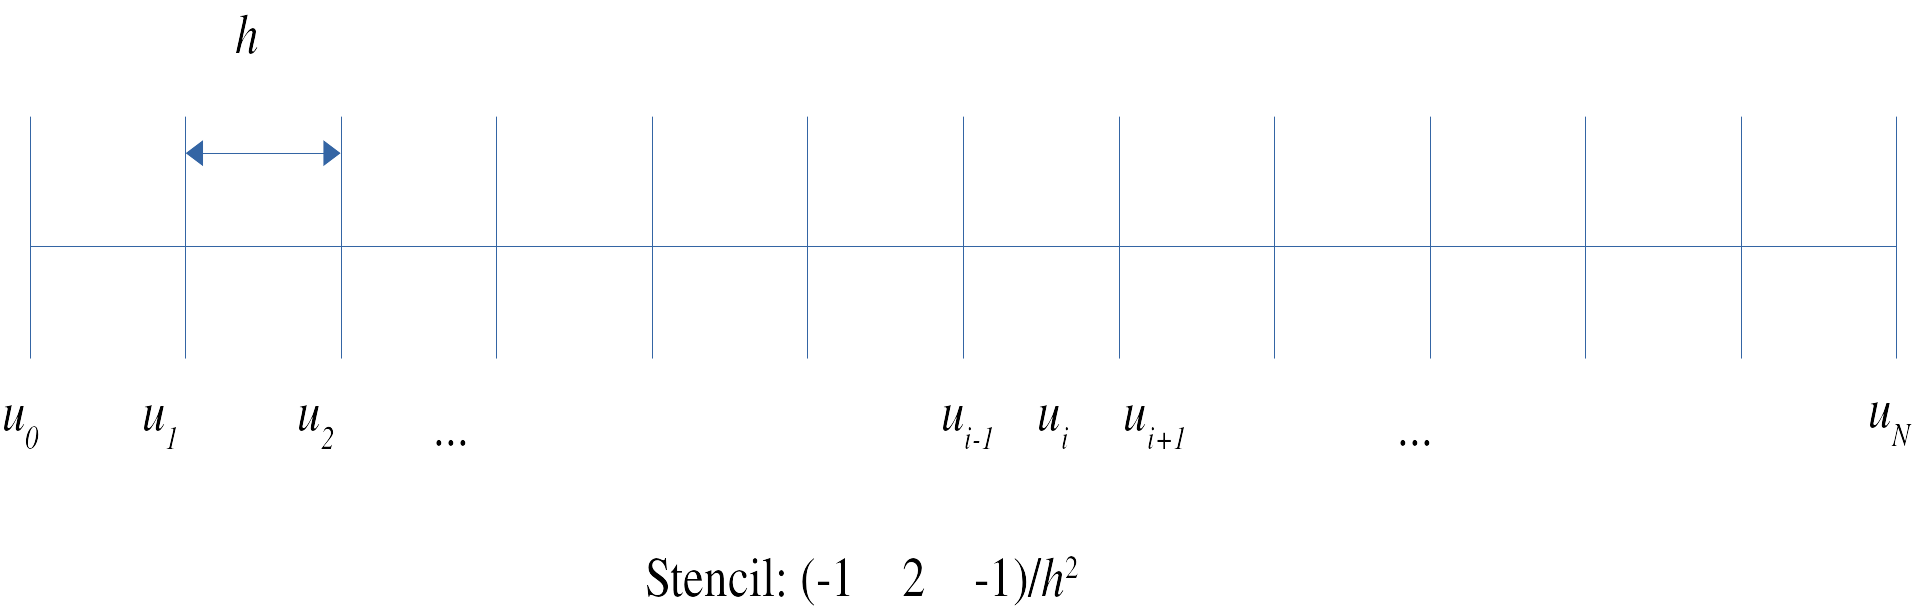
\includegraphics[width=0.7\textwidth]{../figures/1DFDPoisson}
\end{center}
\eq{
\frac{1}{h^2}\begin{bmatrix}
2 & -1 & & & & & & \\
-1 & 2 & -1 & & & & & \\
& -1 & 2 & - 1 & & & & \\
&  & \ddots & \ddots & \ddots & & & \\
& & & & & & & \\
& & & & & -1 & 2 & -1 \\
& & & & & & -1 & 2 \\
\end{bmatrix}
\begin{bmatrix}
u_1 \\
u_2 \\
\\
\vdots \\
\\
\\
u_N \\
\end{bmatrix}
=
\begin{bmatrix}
f_1 \\
f_2 \\
\\
\vdots \\
\\
\\
f_N \\
\end{bmatrix}
}
\end{block}

\end{frame}

\begin{frame}{Motivation and model problems}
\begin{block}{Options for solving the linear system}
\bit
\item Direct methods:
\bit
\item LU decomposition (Gaussian elimination)
\item 
\eit
\eit
\end{block}

\end{frame}

\begin{frame}{Motivation and model problems}
\begin{block}{Solving Poisson with Gaussian elimination}
\bit
\item 
\eit
\end{block}

\end{frame}








\begin{frame}{Motivation and model problems}
\begin{block}{The slide where you show how long it takes to solve the same problem with a bunch of different methods of increasing efficiency}
\bit
\item 
\eit
\end{block}

\end{frame}






\begin{frame}{Motivation and model problems}
\begin{block}{Numerical accuracy}
\bit
\item Discretization accuracy
\item Accuracy of the algebraic solve
\eit
\end{block}

\end{frame}

%%%%%%%%%%%%%%%%%%%%%%%%%%%%%%%%%%%%%%%%%%%%%%%%%%%%%%%%%%%%%%%%%%%%%%%%%%%%%%%%

\section{Basic iterative methods}

\begin{frame}{Basic iterative methods}
\begin{block}{In this section}
\bit
\item Matrix splittings, fixed point methods
\item Basic convergence of splitting methods
\item Jacobi and Gauss-Seidel
\item Application of convergence theory to Jacobi
\item Drawbacks: n dependent convergence that gets very slow as n gets large
\eit
\end{block}

\end{frame}

%%%%%%%%%%%%%%%%%%%%%%%%%%%%%%%%%%%%%%%%%%%%%%%%%%%%%%%%%%%%%%%%%%%%%%%%%%%%%%%%

\section{Krylov subspace methods}

\begin{frame}{Basic iterative methods}
\begin{block}{In this section}
\bit
\item 
\eit
\end{block}

\end{frame}

\end{document}

